\documentclass[10pt,landscape,a4paper]{article}
\usepackage[utf8]{inputenc}
\usepackage{listings}
\usepackage{color}
\usepackage[ngerman]{babel}
\usepackage[T1]{fontenc}
%\usepackage[LY1,T1]{fontenc}
%\usepackage{frutigernext}
%\usepackage[lf,minionint]{MinionPro}
\usepackage{tikz}
\usetikzlibrary{shapes,positioning,arrows,fit,calc,graphs,graphs.standard}
\usepackage[nosf]{kpfonts}
\usepackage[t1]{sourcesanspro}
\usepackage{multicol}
\usepackage{wrapfig}
\usepackage[top=0mm,bottom=1mm,left=0mm,right=1mm]{geometry}
\usepackage[framemethod=tikz]{mdframed}
\usepackage{microtype}
\usepackage{pdfpages}

\usepackage{graphicx}
\graphicspath{ {./images} }

\definecolor{dkgreen}{rgb}{0,0.6,0}
\definecolor{gray}{rgb}{0.5,0.5,0.5}
\definecolor{mauve}{rgb}{0.58,0,0.82}

\lstset{frame=tb,
  language=Java,
  aboveskip=3mm,
  belowskip=3mm,
  showstringspaces=false,
  columns=flexible,
  basicstyle={\small\ttfamily},
  numbers=none,
  numberstyle=\tiny\color{gray},
  keywordstyle=\color{blue},
  commentstyle=\color{dkgreen},
  stringstyle=\color{mauve},
  breaklines=true,
  breakatwhitespace=true,
  tabsize=3,
  basicstyle = \footnotesize
}

\let\bar\overline



\begin{document}
%\footnotesize
\small
\begin{multicols*}{4}
\section{Time Complexity}
{Master's theorem for $T(n) = aT(\frac{n}{b}) + f(n)$ where $a \geq 1$ and $b > 1$} \\
Let $c_{crit} = log_b(a)$ and if $f(n) = \theta(n^c)$
\begin{enumerate}
    \item {If $c < c_{crit}$ then $T(n) = \theta(n^{c_{crit}})$} 
    \item {If $c = c_{crit}$ then $T(n) = \theta(n^clog(n))$} 
    \item {If $c > c_{crit}$ then $T(n) = \theta(f(n))$} 
    \item {If $f(n) = \theta(n^{c_{crit}}log^k(n))$, then $T(n) = \theta(n^{c_{crit}}log^{k+1}(n))$} 

\end{enumerate}

\section{Sorting}
\subsection{Bubblesort}
Time complexity: $\Omega({n})$ $\theta(n^2)$ $O(n^2)$ \\
Invariant: At the end of iteration \texttt{j}, the biggest \texttt{j} items are correctly sorted in the final \texttt{j} positions of the array.

\subsection{SelectionSort}
Time complexity: $\Omega({n^2})$ $\theta(n^2)$ $O(n^2)$ \\
Invariant: At the end of iteration \texttt{j}: the smallest \texttt{j} items are correctly sorted in the first \texttt{j} positions of the array.

\subsection{InsertionSort}
Time complexity: $\Omega({n})$ $\theta(n^2)$ $O(n^2)$ \\
Invariant: At the end of iteration \texttt{j}: the first \texttt{j} items of the array are sorted in order.

\begin{lstlisting}
   for (x = 1 to arr.len):
	j = x - 1
	store = arr[x]
	while(j >= 0 && arr[j] > store):
		arr[j + 1] = arr [j]
		j--
	arr[j+1] = store
\end{lstlisting}

\subsection{QuickSort}
Time complexity: $\Omega({nlog(n)})$ $\theta(nlog(n))$ $O(n^2)$ $O(nlog(n))$ (for paranoid QuickSort)  \\
Invariant: For every \texttt{i < low}: \texttt{B[i] < pivot} and for every \texttt{j > high}: \texttt{B[j] > pivot}.
Duplicates: Use three-way partition to store duplicates.

\subsection{MergeSort}
Time complexity: $\Omega({nlog(n)})$ $\theta(nlog(n))$ $O(nlog(n))$ \\
Invariant: At the end of each loop, the subarrays are sorted.

\subsection{QuickSelect}
Time complexity: $\Omega(n)$ $\theta(n)$ $O(n^2)$ \\ 
Invariant: For every \texttt{i < low}: \texttt{B[i] < pivot} and for every \texttt{j > high}: \texttt{B[j] > pivot}.


\subsection{TopoSort}
Time complexity: $O(V+E)$


% Trees section
\section{Trees}

\subsection{Binary Search Tree (BST)}
Only has 2 children per node. Left child is smaller than parent. Right child is larger than parent. \\
Operations: $O(log(n))$ / $O(n)$ (balanced)

\subsection{AVL Tree}
Maximum height between two children tree is 1. \\
Operations: $O(log(n))$ \\
\textbf{Left Rotation:} \\
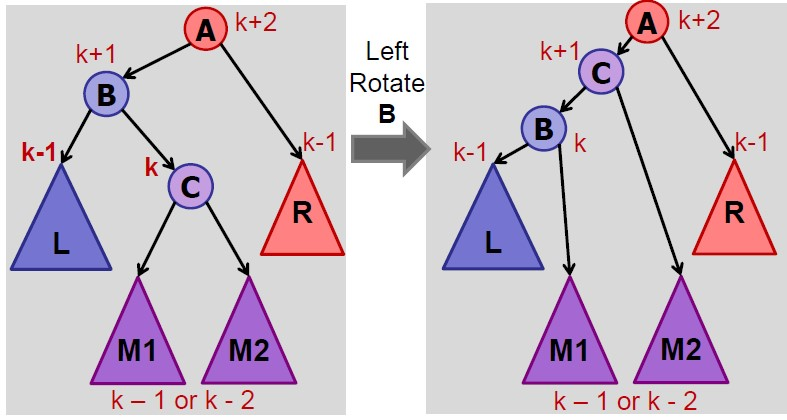
\includegraphics[width = 6cm]{left-rotate} \\
\textbf{Right Rotation:} \\
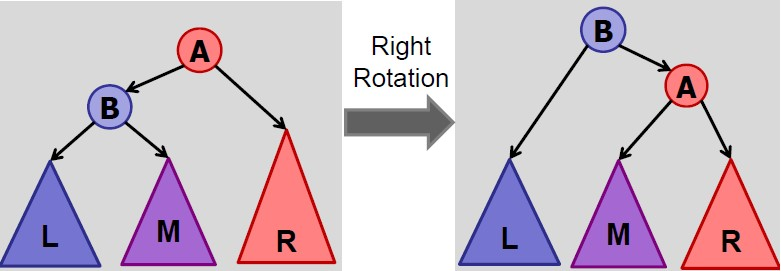
\includegraphics[width = 6cm]{right-rotate} \\
Insertion Max Rotations: 2 \\
Deletion Max Rotations: $log(n)$ \\
Invariant: \texttt{|height(u) - height(v)| < 2} if \texttt{v} and \texttt{u} are sibling nodes. \texttt{|height(u) - height(v)| > 0} if \texttt{u} is the parent node of \texttt{v}.

\subsection{Order Statistics (Rank finding)}
AVL Tree augmented with a \texttt{weight} property in each node. \\
Updating weights on rotate: $O(1)$ \\

\begin{lstlisting}
    rank = weight(node.right) + 1
    while(node != null && node.parent != null):
	    if (node.parent.left == node):
		    rank += weight(node.parent.right) + 1
		    node = node.parent

    FindRanks(currentRank, node, targetRank):
	    check = currentRank + weight(node.left) + 1
	    if (check == targetRank):
		    return node
	    elif (check < targetRank):
		    return FindRanks(currentRank, node.right, targetRank)
	    else:
		    return FindRanks(currentRank, node.left, targetRank)
\end{lstlisting}

\subsection{Interval Trees}
Store the maximum value of entire subtree under a node as a parameter. Update \texttt{max} during rotations by taking \texttt{Math.max} of all children under the two nodes being swapped. \\
\textbf{Time complexity: $O(log(n))$} \\
\begin{lstlisting}
    interval-search(x)
        c = root;
        while (c != null and x is not in c.interval) do
            if (c.left == null) then
                c = c.right;
            else if (x > c.left.max) then
                c = c.right;
            else c = c.left;
                return c.interval;
\end{lstlisting}

\subsection{1D Range Finding}
All leaves hold the value, each internal node \texttt{v} stores the \texttt{MAX} of any leaf in the left sub-tree. \\
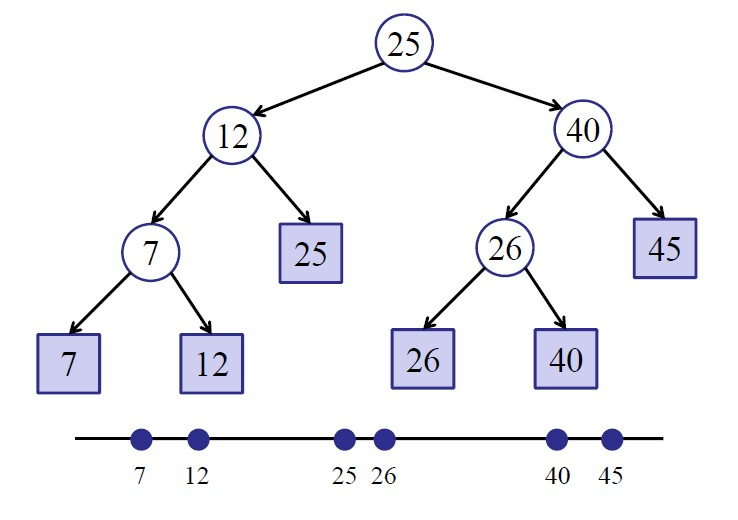
\includegraphics[width = 6cm]{1d-range} \\\\
\textbf{Operations}: \\
\begin{tabular}{p{2cm} p{3.5cm}}
    \verb!findSplit!        & Finds the node to start searching. \\
    \verb!traverseLeft!     & Traverse the left subtree after findSplit. \\
    \verb!traverseRight!    & Traverse the right subtree after findSplit.\\
\end{tabular}\\
\textbf{Complexity}: \\
\begin{tabular}{p{2cm} p{3.5cm}}    
    \verb!Query!    & $O(k + log(n))$ \\
    \verb!Build!    & $O(nlog(n))$ \\
    \verb!Space!    & $O(n)$ \\
\end{tabular}

\subsection{(a, b) trees}
An (a, b) tree has a bound of $2 \le a \le \frac{b+1}{2}$.\\\\
\textbf{Rules:}\\\\
\begin{tabular}{c|c|c|c|c}

    Node Type   &   \multicolumn{2}{|c|}{\#Keys} &  \multicolumn{2}{|c}{\#Children} \\
    {}          &   Min     &   Max            &    Min     &   Max \\
    \hline
    Root        &   1       &   b - 1           &   2       &   b   \\
    \hline
    Internal    &   a - 1   &   b - 1           &   a       &   b   \\
    \hline
    Leaf        &   a - 1   &   b - 1           &   0       &   0   \\

    
\end{tabular}

\section{Hashing}

\section{Heaps}

\section{Graphs}

\section{Dynamic Programming}
%\input{inhalt/graphalgo}
%\input{inhalt/bool}
%\input{inhalt/formeln}
\end{multicols*}
\end{document}